\begin{frame}
    \frametitle{Server im Rechenzentrum}
    \begin{center}
      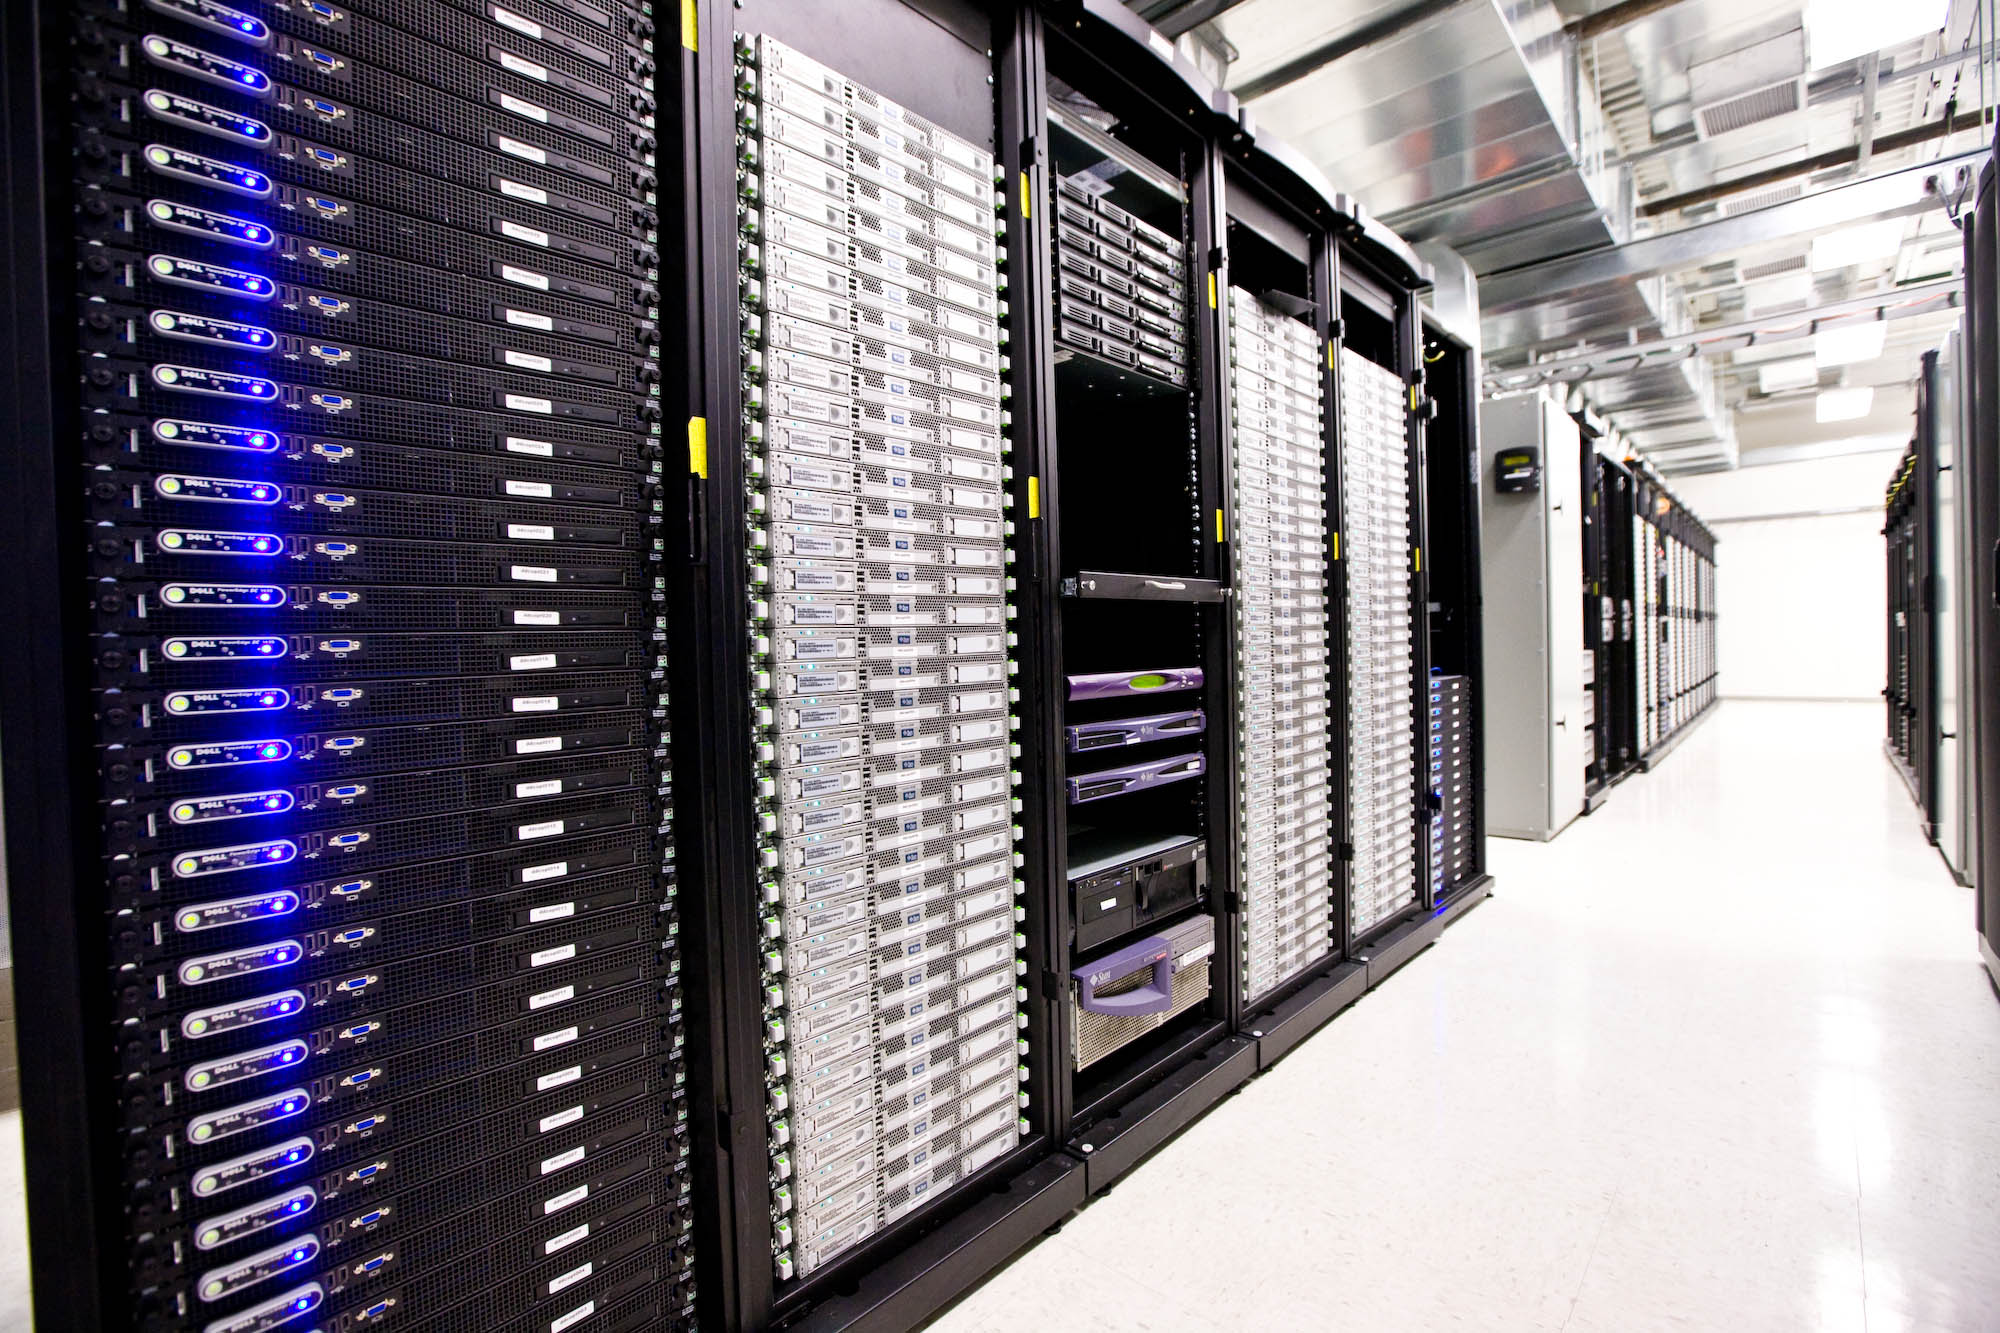
\includegraphics[height=5cm]{../../img/data_center.jpg}
    \end{center}
\end{frame}

\note{Server stehen üblicherweise in großen Rechenzentren überall auf der Welt verteilt. Die abgebildeten Schränke heißen Racks und jeder Einschub ist ein Server, d.h. ein Computer, der keinen Bildschirm und keine Maus hat, dafür aber einen Netzwerkanschluss. Ein Server kann einen oder mehrere Dienste anbieten, z.B. eine abrufbare Website, einen Emailanbieter, einen Kommunikationsdienst für eine App etc. Große Dienste, wie Google oder Whatsapp sind üblicherweise auf viele Server in unterschiedlichen Rechenzentren verteilt.}

\begin{frame}
    \frametitle{Internetknoten (Router)}
    \begin{center}
      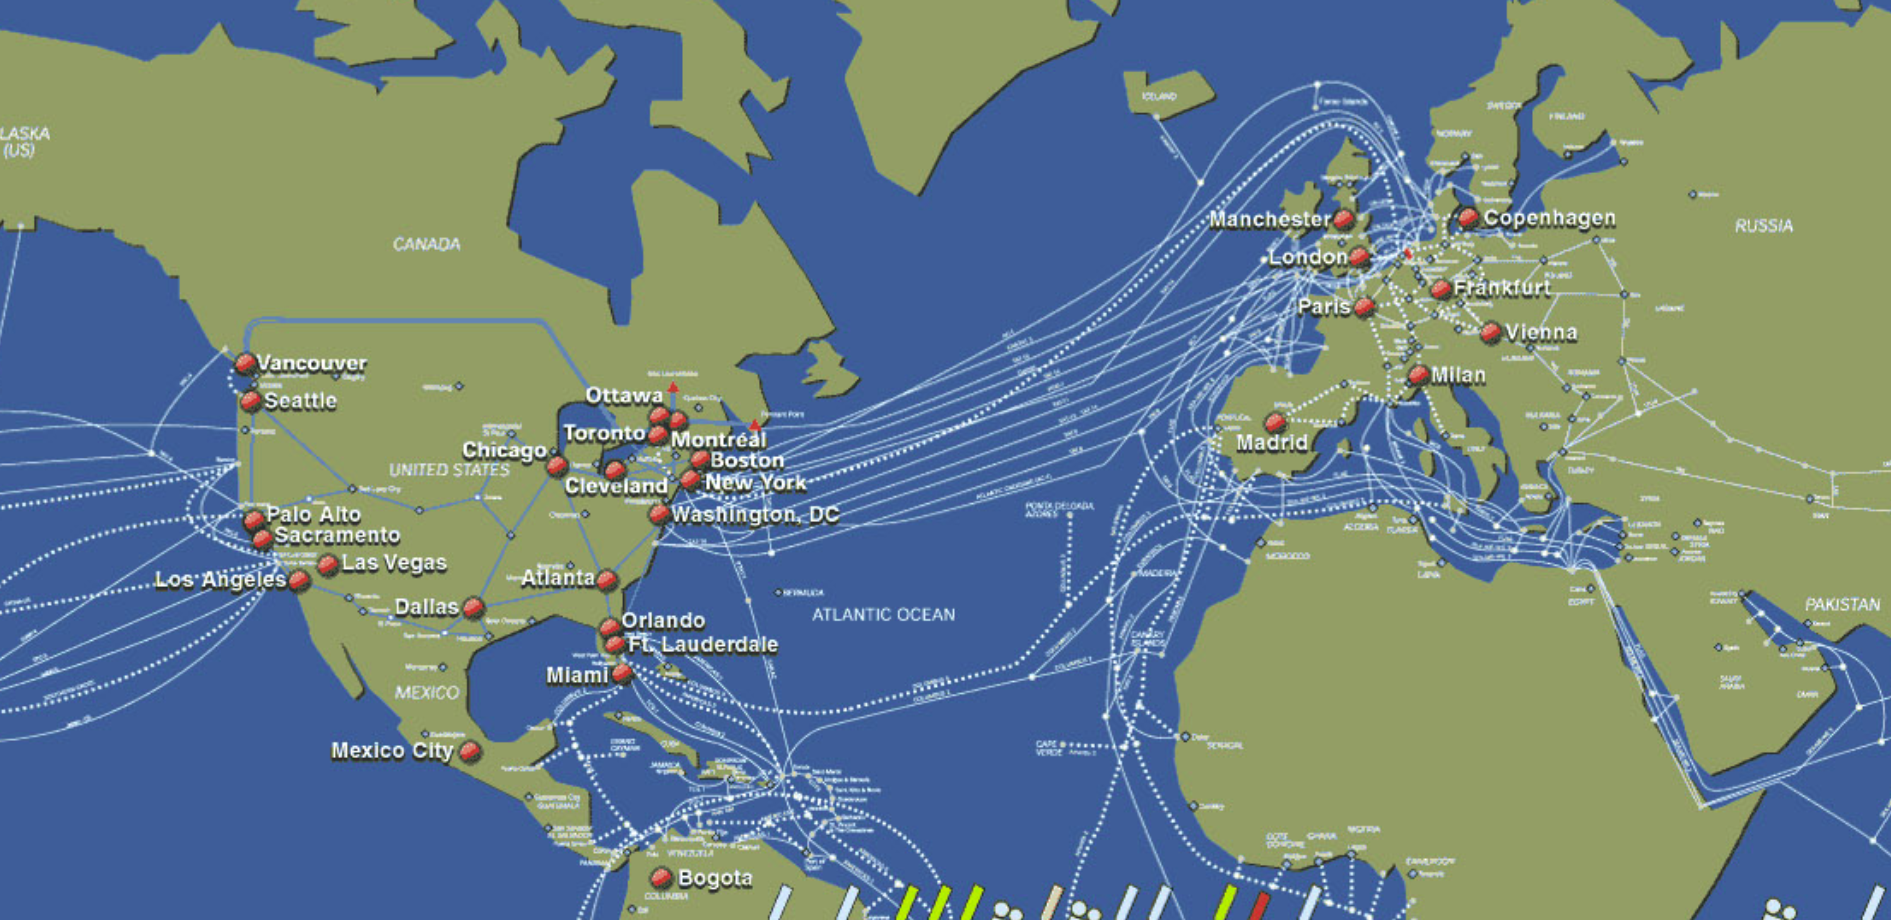
\includegraphics[height=5cm]{../../img/internet_cable_map.png}
    \end{center}
\end{frame}

\note{Das Versenden einer Anfrage (z.B. der Aufruf einer Website) übers Internet ist vergleichbar mit dem Verschicken eines Postpakets, man gibt es an der lokalen Post ab und dann wird es über kleinere und größere Paketverteilstationen - ggf. übers Meer - zu seinem Empfänger gebracht. Diese Verteilzentren nennen sich im Internet Router oder Switches und sind dafür da, dass die Internetpakete nach vielen Schritten vom Nutzer zum Server und im Falle einer Antwort auch wieder zurückkommen.}

\begin{frame}
    \frametitle{Internetknoten (DE-CIX in Frankfurt)}
    \begin{center}
      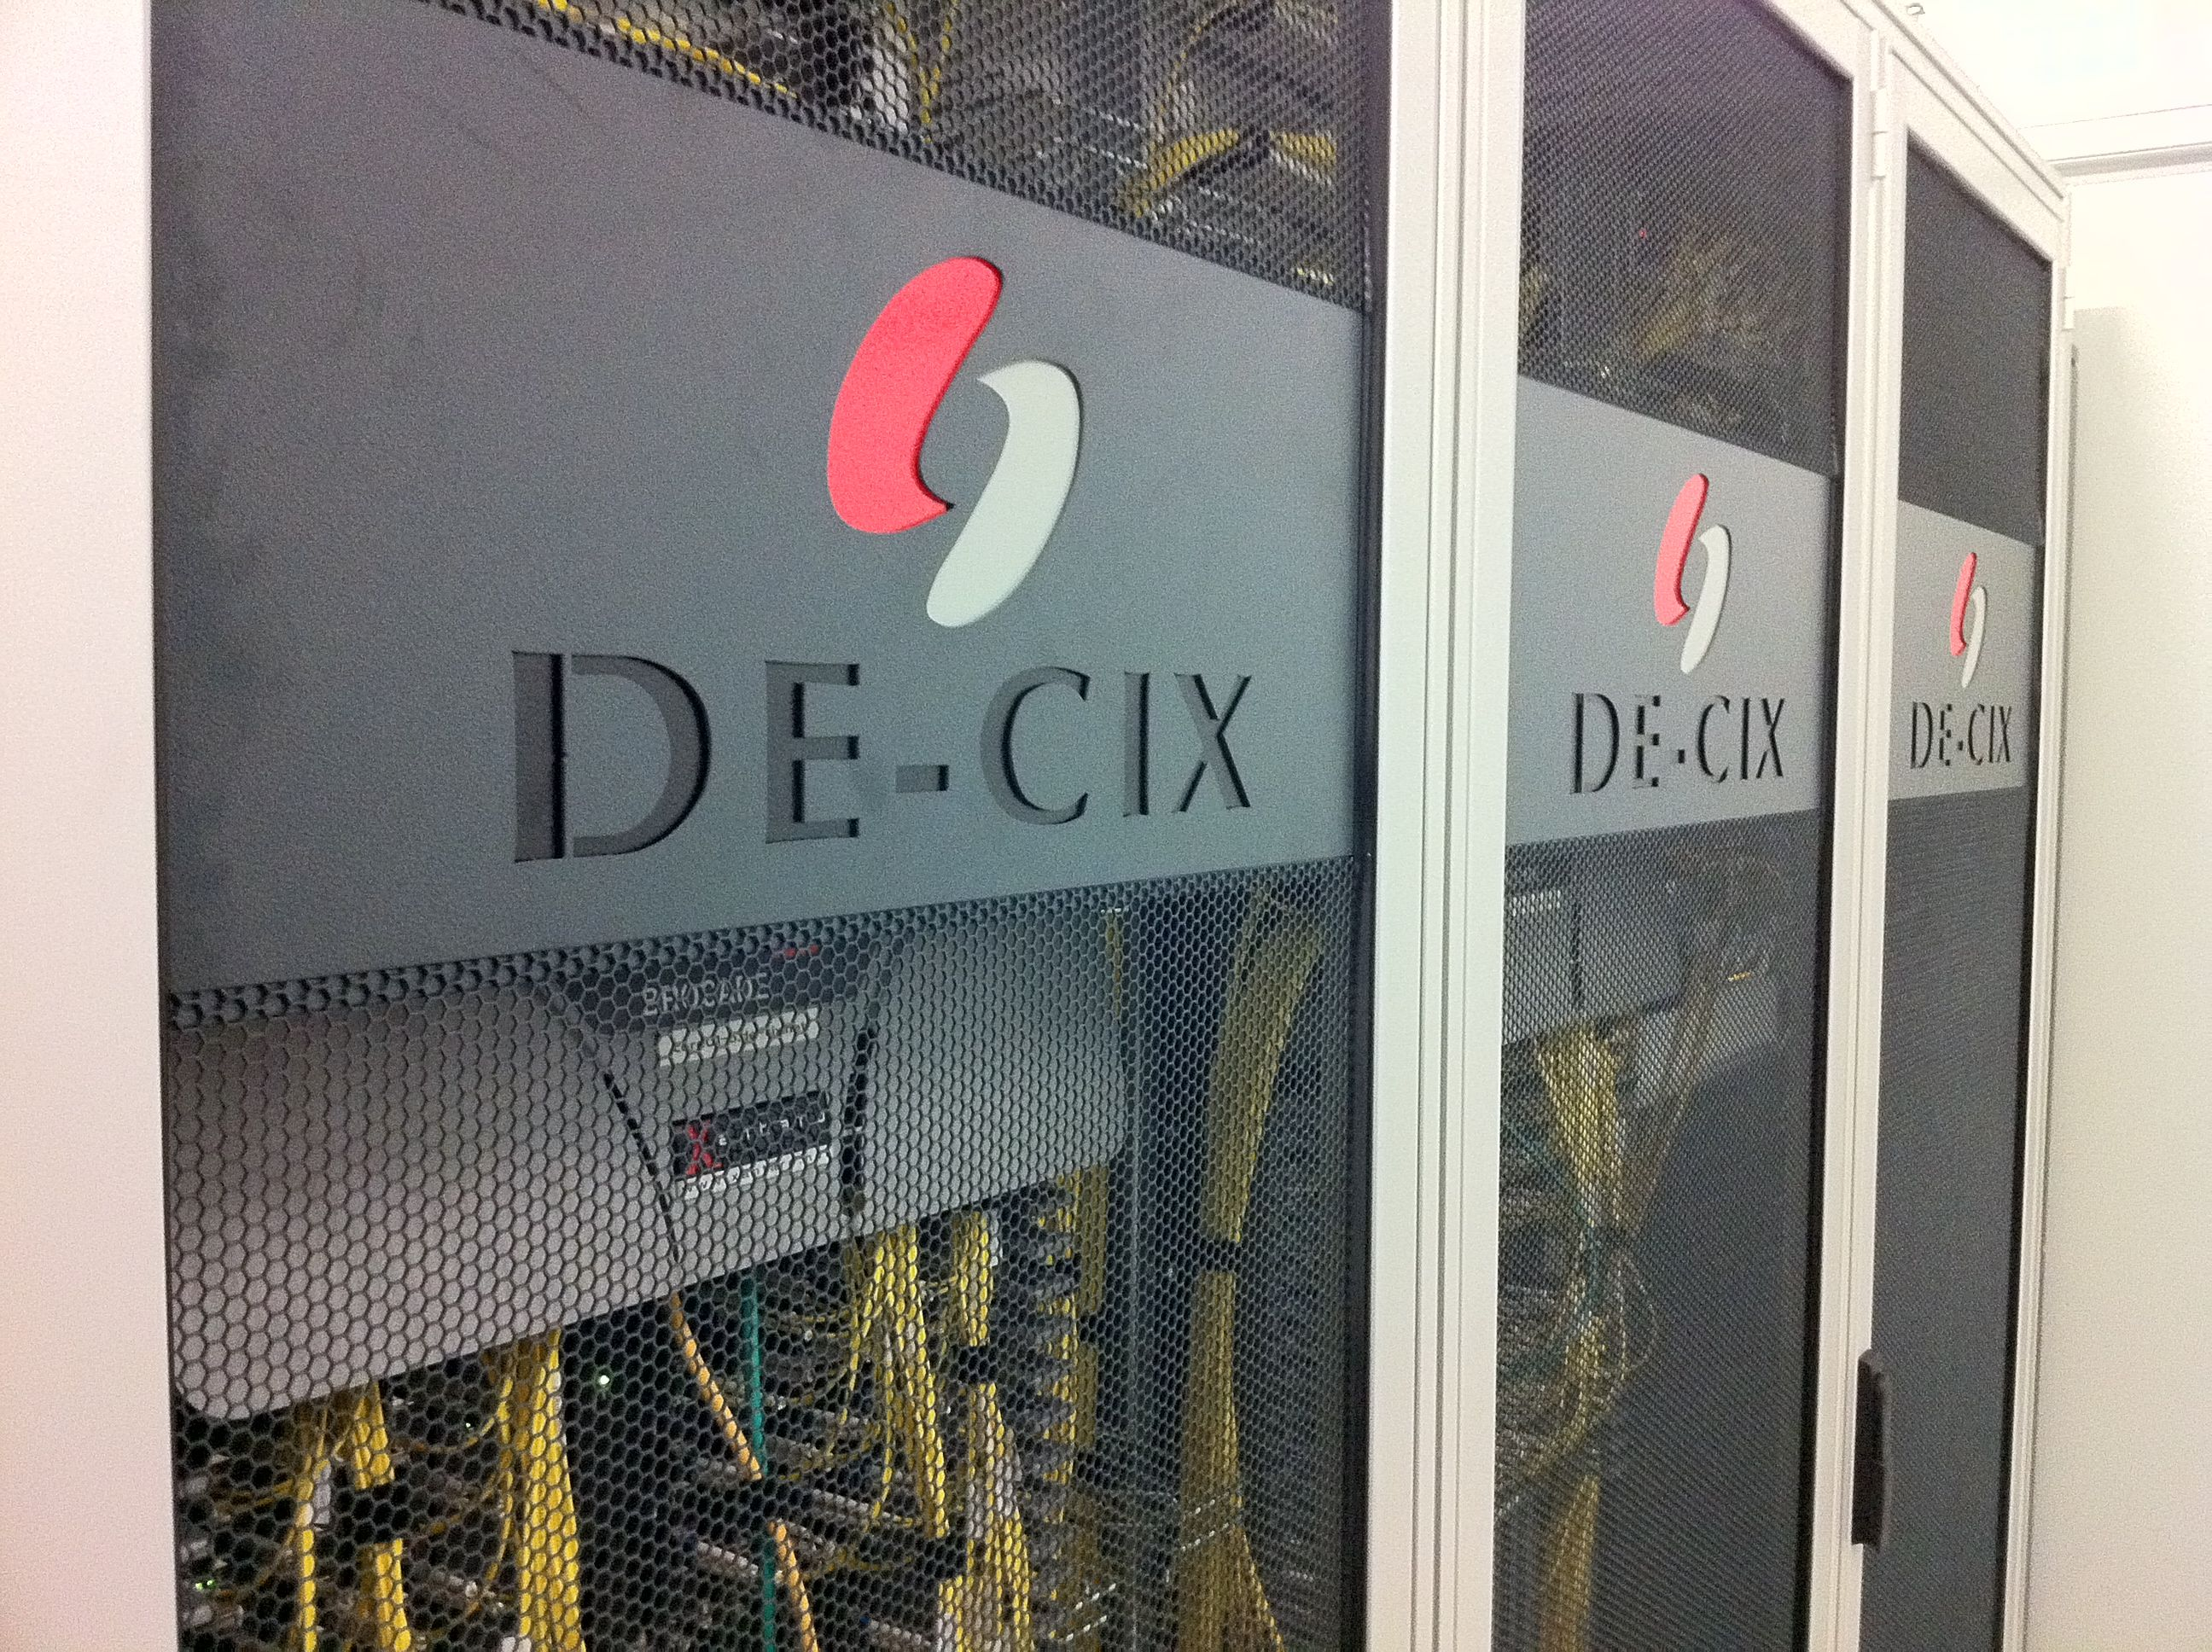
\includegraphics[height=5cm]{../../img/de_cix.jpg}
      \\{\small \href{https://de.wikipedia.org/wiki/DE-CIX\#/media/File:DE-CIX\_GERMANY\_-\_Switch\_Rack\_\%286218137120\%29.jpg}{Grafik}: \href{https://creativecommons.org/licenses/by-sa/2.0/}{\cc{by-sa} Stefan Funke}}
    \end{center}
\end{frame}

\note{Der abgebildete Verteilknoten ist der DE-CIX in Frankfurt, der Größte der Welt, der nicht aus einem sondern aus ganz vielen Routern besteht.}
